\section{Results}

\begin{frame}
        \centering
        \huge Results
\end{frame}

\begin{frame}
	\begin{figure}
		\centering
		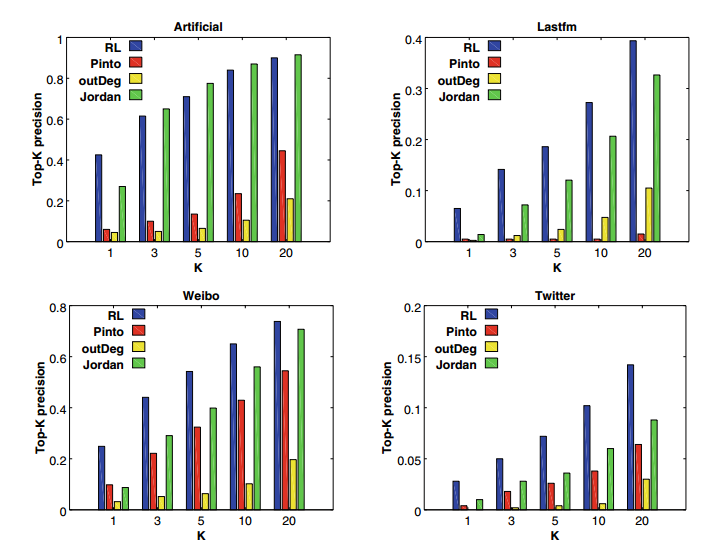
\includegraphics[scale=0.5]{fullcascade.png}
		\caption{Source detection with full cascades}
	\end{figure}
\end{frame}

\begin{frame}
	\begin{figure}
		\centering
		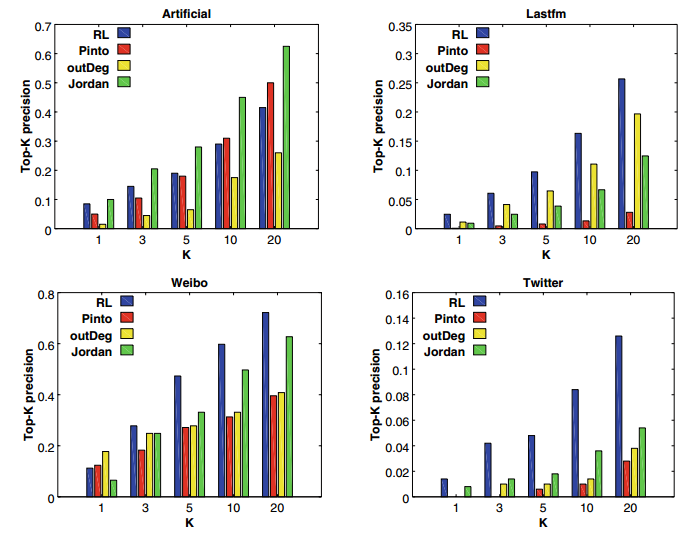
\includegraphics[scale=0.5]{partialcascade.png}
		\caption{Source detection with partial cascades (20\%)}
	\end{figure}
\end{frame}

\begin{frame}
	\begin{figure}
		\centering
		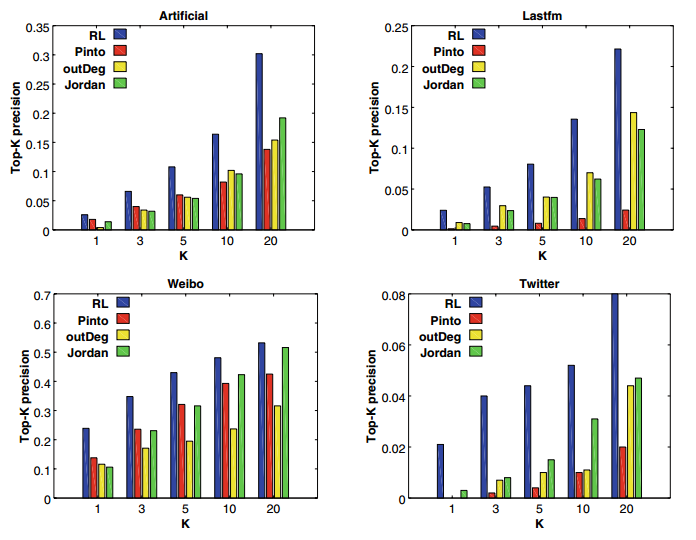
\includegraphics[scale=0.5]{partiallyobserved.png}
		\caption{Source detection with partially observed cascades (20\%)}
	\end{figure}
\end{frame}

\begin{frame}
	\begin{figure}
		\centering
		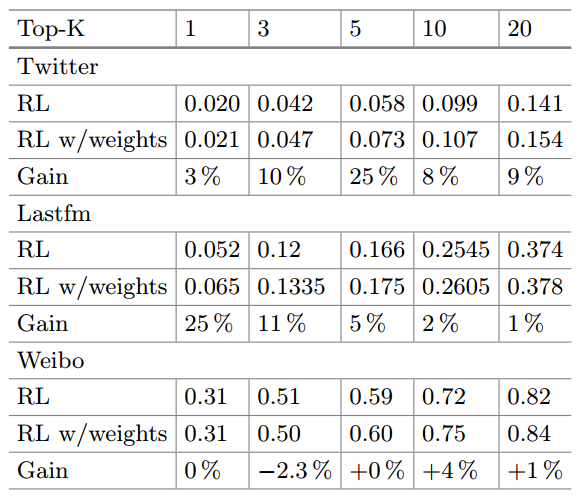
\includegraphics[scale=0.5]{userweights.png}
		\caption{Source detection with user weights}
	\end{figure}
\end{frame}

\begin{frame}
	\begin{figure}
		\centering
		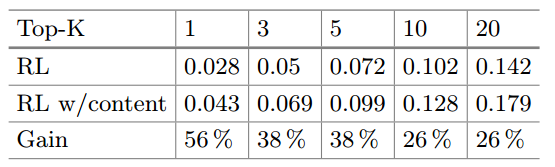
\includegraphics[scale=0.5]{contentintegration.png}
		\caption{Source Detection with Content Integration on the Twitter dataset}
	\end{figure}
\end{frame}